\problemname{Lego Building Competition}
\noindent
You and your arch-enemy Gohu have participated in a Lego building competition.
You have built many towers of varying heights and beauty along the $x$-axis and are now waiting for the judges to arrive.
The scoring will be as follows: if one of your towers has a beauty rating of $f$ and is $h$ Lego bricks high, you will get $f \cdot h$ points for the tower.

The Lego building competition is a world-renowned event, and as such, many drones are flying back and forth to film all the beautiful towers.
To prevent the drones from crashing into the towers (thereby knocking down all the bricks above and including the brick they hit), the film crew has placed numerous radio masts of different heights along the $x$-axis.
A drone can move one unit up or down for each unit it moves forward and will always move to stay as close to the ground as possible (to get good shots of the towers) without ever going below a mast.
In the images below, you can see illustrations of how the masts affect the drones' paths.

Suddenly, the film crew looks away!
You decide to quickly remove some masts from the line so that the drones will start crashing into the towers.
If a drone, after the masts are removed, starts flying at height $h$ in a column that has a tower with at least height $h$, the drone crashes into the tower.
The new height of the tower then becomes $h - 1$.
Its beauty rating does not change.
If a drone crashes into a tower when it is at height $h$, the tower's new height becomes $h - 1$, but its beauty rating remains the same.
It is guaranteed that the masts are initially placed so that drones do not crash into any towers.

Which masts should you remove to maximize your profit (the difference between your points and Gohu's)?

\section*{Input}
The first line contains three integers $A, B, M$ ($1 \leq A, B, M \leq 2000$): the number of towers you built, the number of towers Gohu built, and the number of masts.

This is followed by $A$ lines where each line contains integers $x, f, h$ ($1 \leq x \leq 10^6, 1 \le f \le 100, 1 \leq h \leq 10000$) -- the position, beauty rating, and height of one of your towers.

Next, there are $B$ lines where each line contains integers $x, f, h$ ($1 \leq x \leq 10^6, 1 \le f \le 100, 1 \leq h \le 10000$) -- the position, beauty rating, and height of one of Gohu's towers.

Finally, there are $M$ lines where each line contains integers $x, h$ ($1 \leq x \leq 10^6, 1 \leq h \leq 10000$) -- the position and height of one of the masts.

No towers will have the same $x$ value as each other, and neither will the masts.
However, masts can have the same $x$ position as towers.

\section*{Output}
Print a single integer: the maximum value $(\text{your points}) - (\text{Gohu's points})$ you can achieve if you optimally choose which masts to remove.

\section*{Points}
Your solution will be tested on several test case groups.
To get the points for a group, it must pass all the test cases in the group.

\noindent
\begin{tabular}{| l | l | l |}
  \hline
  \textbf{Group} & \textbf{Point value} & \textbf{Constraints} \\ \hline
  $1$   & $23$       & Masterna har lägre x-koordinat än tornen. \\ \hline
  $2$   & $10$       & $A,B,M \leq 8$\\ \hline
  $3$   & $22$       & $A,B,M \leq 100$  \\ \hline
  $4$   & $45$       & No additional constraints. \\ \hline
\end{tabular}

\section*{Explanation of Samples}
In all images, your towers are shown in blue and Gohu's towers in red.

\begin{figure}[!h]
  \centering
  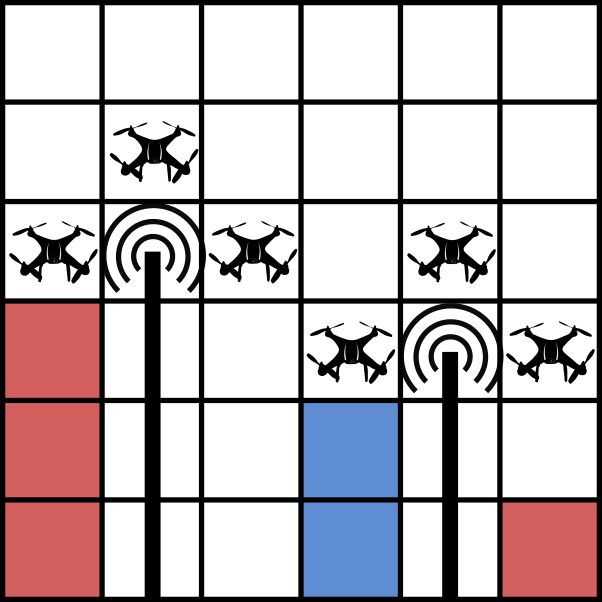
\includegraphics[width=4cm]{sample1.png}
  \caption{Example case 1}
\end{figure}
In the first example case, it is optimal to remove only the first mast.
The drones will then start flying at height $1$ in the column with the leftmost tower, which will be completely destroyed.
After that, you have $2$ points and Gohu has $0 + 1$ points, with a difference of $1$ point.

\begin{figure}[!h]
  \centering
  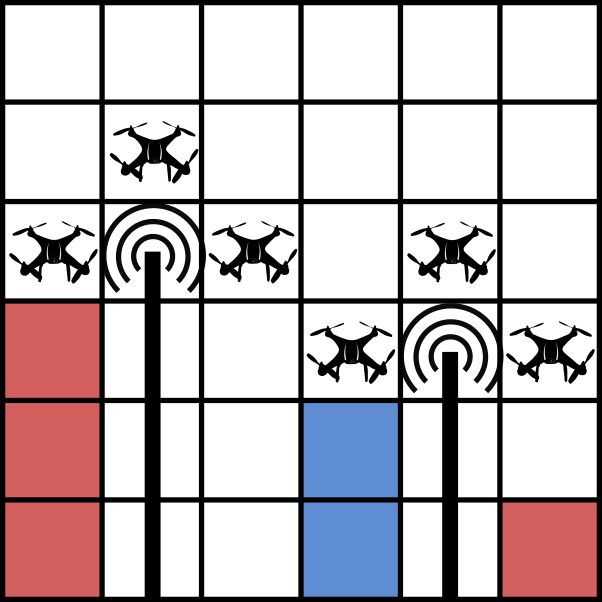
\includegraphics[width=6cm]{sample1.png}
  \caption{Example case 2}
\end{figure}
In the second example case, the best you can do is to remove the second and third masts.
The drone will then fly at heights $5$, $6$, $5$, $4$, $3$, $4$, $5$, $6$, $7$, $8$.
The first, third, and fourth towers will therefore lose a brick, while the second and last towers are not affected at all.
The towers will have heights $4$, $5$, $3$, $3$, $6$.

After that, you have $500 + 30 + 120 = 650$ points and Gohu has $400 + 30 = 430$ points, with a difference of $220$ points.

\begin{figure}[!h]
  \centering
  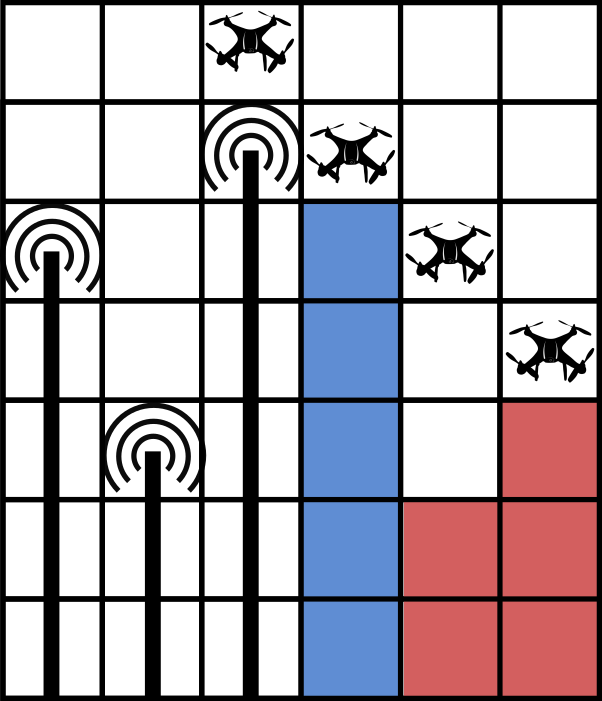
\includegraphics[width=4cm]{sample3.png}
  \caption{Example case 3}
\end{figure}
In the third example case, it is optimal to remove the second and third masts.
After that, you have $20$ points and Gohu has $9$ points, with a difference of $11$ points.
